%%%%%%%%%%%%%%%%%%%%%%% Preamble to Document %%%%%%%%%%%%%%%%%%%%%%% 
% Set type of document to article
\documentclass{article}

% Encoding for document, allows for use of characters beyond ASCII
\usepackage[utf8]{inputenc}

% Math symbols
\usepackage{amsmath}

% Change margins
\usepackage[margin=1in]{geometry}

% Control page headers and footers
\usepackage{fancyhdr}
\pagestyle{fancy}

% Change text colors
\usepackage[dvipsnames,table]{xcolor}

% Produce hypertext links in the document
\usepackage{hyperref}

%Write Chemical Equations: 
\usepackage{mhchem}

%Bibliography Resources
\usepackage[sorting = none]{biblatex}
\addbibresource{references.bib}

% Add colored boxes around text
\usepackage[most]{tcolorbox}
% Define examples 
\newtcbtheorem[auto counter,number within=section]{ex}%
  {Example}{fonttitle=\bfseries\upshape, fontupper=\slshape,
     arc=0mm, colback=MidnightBlue!5!white,colframe=MidnightBlue!75!black, width=10cm}{example}

\newtcbtheorem[auto counter]{acta}%
  {Activity}{fonttitle=\bfseries\upshape, fontupper=\slshape,
     arc=0mm, colback=Periwinkle!5!white,colframe=Periwinkle!75!black, width=15cm}{actA}

% My new colors
\definecolor{myBlack}{rgb}{0,0,0}
\definecolor{myWhite}{rgb}{1,1,1}
\definecolor{myNewColor}{rgb}{0.26,0.90,0.47}

% Make it so hyperlinks are different colors 
\hypersetup{
    colorlinks,
    linkcolor={black!100!black},
    citecolor={blue!50!black},
    urlcolor={blue!80!black}
}

% Set the default indentation to be none
\setlength\parindent{0pt}

% Control vertical spacing between items in list
\usepackage{enumitem}
\setlist{nosep}

% Wrap text around figure 
\usepackage{wrapfig}

% Insert a pdf
\usepackage{pdfpages} 

% Set the header 
\lhead{MCSB Bootcamp 2019} % Left header 
\chead{Complex Document Preparation \& LaTeX} % Center header
\rhead{\today} % Right header (today's date)

%%%%%%%%%%%%%%%%%%%%%%% Begin Document %%%%%%%%%%%%%%%%%%%%%%% 
\begin{document}

\thispagestyle{empty} % Set the page style to empty
\begin{center}
    \Large
    \textbf{Complex Document Preparation \& LaTeX}\\
    \normalsize
    MCSB Bootcamp\\
    September 12, 2019\\
    Written by: Tessa Morris
\end{center}

\tableofcontents % Print Table of Contents
\newpage % Start a new page 

\section{Introduction}
LaTeX is a document preparation system used to create professional-looking documents. It is used extensively for communication and publication of scientific documents.

\subsection{Objectives}
\begin{enumerate}
    \item The main objective is to get comfortable using LaTeX for homework assignments the first year.
    \item The secondary, and arguably the more important objective is to be able to use LaTeX for manuscripts. 
\end{enumerate}

\subsection{Advantages and Disadvantages of LaTeX}
\textbf{Advantages:}
\begin{enumerate}
    \item Mathematical notation and referencing
    \item Consistent handling of intra-document references and bibliography
    \item Content and style are separated 
    \item Packages to do most anything (can also be a disadvantage)
\end{enumerate}
\textbf{Disadvantages:}
\begin{enumerate}
    \item Collaborative editing can be difficult without the use of git or Overleaf
    \item Some barrier to entry 
\end{enumerate}
\subsection{Advantages and Disadvantages of Overleaf}
\textbf{Advantages}
\begin{itemize}
    \item Easy compiling 
    \item Avoid compatibility issues between different operating systems 
    \item Contains existing templates
\end{itemize}
\textbf{Disadvantages}
\begin{itemize}
    \item Requires internet connection 
    \item It can take longer to compile 
\end{itemize}
\subsection{Specific Objectives}
\begin{enumerate}
    \item Understand LaTeX structure and syntax
    \item Learn notation (e.g. backslashes and brackets)
    \item Add a package 
    \item Change formatting 
    \item Learn the different types of mathematical equation modes (Section \ref{equationSection})
    \item Write mathematical expressions (fractions, square roots, exponents, matrices, ect…) 
    \item Include a figure, label the figure, and reference the figure 
    \item Citations and reference file
    \item Make a table 
    \item Compatibility with Mathematica, Mendeley and other reference managers, Import code from a file 
\end{enumerate}
\newpage
\section{LaTeX Components \& Basic Syntax}

\subsection{LaTeX Document Components}
LaTeX is separates the content of the document from the style. Therefore it is common to create one style of document with the desired appearance and then use that document as a template in future projects. Accordingly, many scientific journals create and require authors to use their LaTeX manuscript templates. \\

A .tex file has two components: the \textbf{preamble} and the \textbf{body of the document}. 
\begin{itemize}
    \item The \textbf{preamble} is where the document type is defined, packages are loaded, and parameters are set. For example, the first line of code in Figure \ref{fig:blankDocument} declares the type of document (i.e. class), which controls the overall appearance of the document. In this case, the class is article, the simplest and most common LaTeX class. The preamble ends and the body of the document begins with \verb!\begin{document}!. 
    \item The \textbf{body of the document} is the content of the document and is enclosed inside \verb!\begin{document}! and \verb!\end{document}!.
\end{itemize}

%Follow Activity \ref{actA:helloworld} to change the body of the text to display ``Hello World!'' as in Figure \ref{fig:helloWorld}. 

\subsection{Starting From a Blank Project}
One of the advantages of \href{www.overleaf.com}{Overleaf} is that it has multiple templates, as well as the ability to upload an existing project and create a new blank document (Figure \ref{fig:blankDocument}). Once familiar with LaTeX, it is recommended to use a template that has the desired style for your project. However, starting from a blank project can makes it easier to focus on learning the basic structure and syntax (Activity \ref{actA:newdoc}). 

\begin{figure}[h]
    \centering
    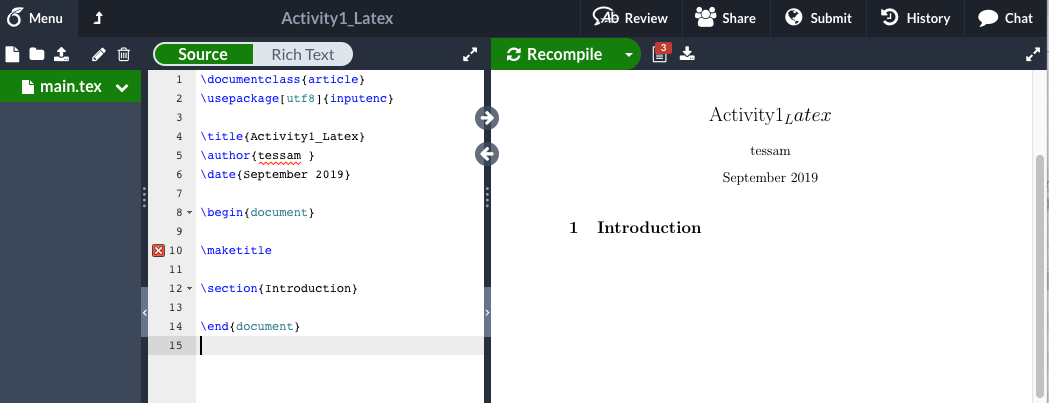
\includegraphics[width=0.9\textwidth]{blankDocument.png}
    \caption{A blank document automatically generated by Overleaf. Overleaf displays the \color{OliveGreen}\textbf{Source }\color{black} or the .tex code on the left side of the screen and the compiled .pdf on the right side of the screen.}
    \label{fig:blankDocument}
\end{figure}

\begin{figure}[h]
    \centering
    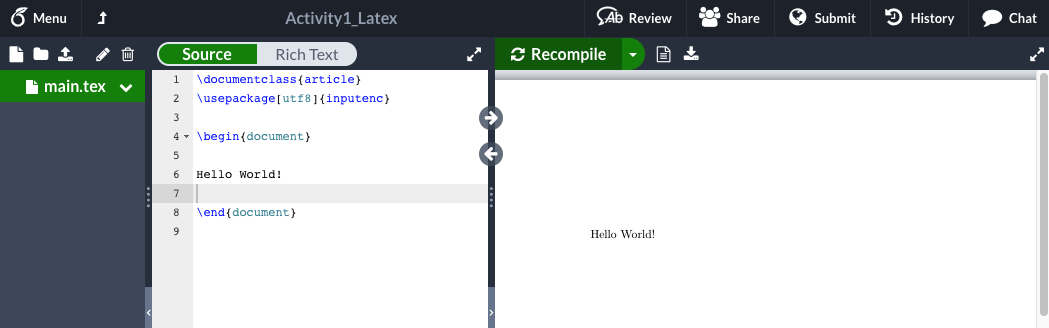
\includegraphics[width=0.9\textwidth]{helloWorld.png}
    \caption{Display ``Hello World!'' using LaTeX. }
    \label{fig:helloWorld}
\end{figure}


\begin{center}
\begin{acta}{Create a New Blank Project \& Display ``Hello World!''}{newdoc}
\normalfont
\begin{enumerate}
    \item Open a new internet browser tab,  navigate to \url{www.overleaf.com}, and login. 
    \item Select \color{OliveGreen}\textbf{New Project }\color{black} and then \color{OliveGreen}\textbf{Blank Project}\color{black}.
    \item Once you have named and created your project it should similar to Figure \ref{fig:blankDocument}. \\
\end{enumerate}

At this stage, the document contains the title and a section named ``Introduction''.\\

Overleaf creates the title in the following way:
\begin{itemize}
    \item \verb!\title! Project Name (Activity\_Latex in Figure \ref{fig:blankDocument})\\
    Note: There is an error (indicated by the red x on line 10) because the underscore indicates a subscript in math mode of LaTeX (Section \ref{equationSection}). Math mode is not properly indicated and therefore, there is a compilation error. 
    \item \verb!\author! Your User Name (tessam in Figure \ref{fig:blankDocument})
    \item \verb!\date! Current Month Current Year (September 2019 in Figure \ref{fig:blankDocument})\\
\end{itemize}


Change the document to display ``Hello World'' as in Figure \ref{fig:helloWorld}. 
\begin{enumerate}
    \item In the body of the document, comment out the existing text (\verb!\maketitle!  and  \texttt{\textbackslash section\{Introduction\}}) by adding a \% symbol (Section \ref{commentsSection}).
    \item Type \texttt{Hello World!} in the body of the document. 
    \item Recompile. Your rendered document should look like that in Figure \ref{fig:helloWorld}. 
    \item You can also comment out the commands in the preamble that create the title (See Activity \ref{actA:newdoc}) as the title is no longer rendered. 
\end{enumerate}
\end{acta}
\end{center}



% \begin{center}
% \begin{acta}{Use LaTeX to display ``Hello World!''}{helloworld}
% \normalfont
% The Blank Project automatically generated by Overleaf (Figure \ref{fig:blankDocument}) contains both a title and section called ``Introduction''. We would like for the document to simply display ``Hello World'' instead. 
% \begin{enumerate}
%     \item In the body of the document, comment out the existing text (\verb!\maketitle!  and  \texttt{\textbackslash section\{Introduction\}}) by adding a \% symbol (Section \ref{commentsSection}).
%     \item Type \texttt{Hello World!} in the body of the document. 
%     \item Recompile. Your rendered document should look like that in Figure \ref{fig:helloWorld}. 
%     \item You can also comment out the commands in the preamble that create the title (See Activity \ref{actA:newdoc}) as the title is no longer rendered. 
% \end{enumerate}
% \end{acta}
% \end{center}

\subsection{Comments}\label{commentsSection}
As with any code you are writing, it can often be useful to include comments. To make a comment in LaTeX add a \% symbol before the comment text (Example \ref{example:comment}). 

\begin{center}
\begin{ex}{Adding a Comment}{comment}
\normalfont
  \texttt{\% This is a comment}
\end{ex}
\end{center}

In Overleaf, the keyboard shortcut to comment out a line of code is Control (or Command) + Slash (/)

\subsection{Simple Text Formatting}
Simple formatting includes bolding, italicising and underlining text (Example \ref{example:emphasis}), as well as, changing the font size (Example \ref{example:size})

\begin{center}
\begin{ex}{Changing the Emphasis}{emphasis}
\normalfont
\textbf{Bold text} using the \texttt{\textbackslash textbf\{$\cdots$\}} command.\\
\textit{Italicise text} using the \texttt{\textbackslash textit\{$\cdots$\}} command.\\
\underline{Underline} text using the \texttt{\textbackslash underline\{$\cdots$\}} command.\\
\end{ex}
\end{center}

\begin{center}
\begin{ex}{Changing the Font Size}{size}
\normalfont
\Huge
\texttt{\textbackslash Huge} \Huge Text \\
    \huge
\texttt{\textbackslash huge} \huge Text \\
    \LARGE 
\texttt{\textbackslash LARGE} \LARGE Text \\
    \Large
\texttt{\textbackslash Large} \Large Text \\
    \large 
\texttt{\textbackslash large} \large Text \\
    \normalsize 
\texttt{\textbackslash normalsize} \normalsize Text (default size) \\
    \small 
\texttt{\textbackslash small} \small Text \\
    \footnotesize 
\texttt{\textbackslash footnotesize} \footnotesize Text \\
    \scriptsize
\texttt{\textbackslash scriptsize} \scriptsize Text \\
    \tiny 
\texttt{\textbackslash tiny} \tiny Text
\normalsize 
\end{ex}
\end{center}

\begin{center}
\begin{acta}{Replicate this Text}{simptext}
\normalfont
How would you replicate the following text, where ``Hello'' is in small font and italicized, ``World!'' is in Huge font, underlined, and bold?:\\
\begin{center}
\small \textit{Hello} \Huge \underline{\textbf{World!}}
\end{center}
\normalsize
\end{acta}
\end{center}

\subsection{Document Sectioning}
LaTeX can organize, number, and index chapters and sections of document. Use the command \texttt{\textbackslash section\{$\cdots$\}} to create a new section (Activity \ref{actA:sec}). 

\begin{center}
\begin{acta}{Add Sections}{sec}
\normalfont
\begin{enumerate}
    \item Add multiple sections using the command \texttt{\textbackslash section\{$\cdots$\}}. 
    \item Change the order of the sections around and see how the numbering changes. 
    \item What happens if you change the command to \verb!\section*!\texttt{\{$\cdots$\}}?
\end{enumerate}
\end{acta}
\end{center}
\subsection{Environments}
Environments are regions in the document that are formatted in a special manner depending on the type of the environment. They start with a \texttt{\textbackslash begin\{$\cdots$\}} command and end with an \texttt{\textbackslash end\{$\cdots$\}} command. Common examples include centering, lists (Section \ref{listSection}), equations (Section \ref{equationSection}), and figures (Section \ref{figureSection}).\\

\begin{center}
\begin{acta}{Test Centering Environment}{cent}
\normalfont
Create a centering environment around the text ``Hello World''.\\
Hint: Start the environment with \verb!\begin{center}!
\end{acta}
\end{center}

\subsection{Packages}
Packages can be used to change the default look of your LaTeX document, or to allow more functionalities. To use the a package a the following line in you preamble \texttt{\textbackslash usepackage\{$\cdots$\}} (Activity \ref{actA:colorpck}). 

\begin{center}
\begin{acta}{Change Text Color}{colorpck}
\normalfont
The package xcolor allows you to manipulate the color in your document. In this activity, we'll use it to simply change the text color. 
\begin{enumerate}
    \item Install \texttt{xcolor} by adding \texttt{\textbackslash usepackage\{xcolor\}} to the preamble. 
    \item Change of the text to red by adding the line \texttt{\textbackslash color\{red\}} in the body of the document. 
\end{enumerate}

You can also define your own text color by defining your color in the preamble. We will use the RGB code (each channel ranging between 0 and 1) to define the colors.
\begin{itemize}
    \item Add the line \texttt{\textbackslash\{myBlack\}\{rgb\}\{0,0,0\}} to the preamble.
    \item Add the line \texttt{\textbackslash\{myWhite\}\{rgb\}\{1,1,1\}} to the preamble.
    \item Add the line \texttt{\textbackslash\{myNewColor\}\{rgb\}\{0.26,0.90,0.47\}} to the preamble.
    \item Call each color as you did before when you changed the color to red.  
\end{itemize}
\end{acta}
\end{center}

\subsection{New Lines}
Leave one full empty line between two paragraphs. Place \verb!\\! at the end of a line to create a new line (but not create a new paragraph).


\subsection{Lists}\label{listSection}
Lists can either be ordered (\texttt{itemize} environment) or unordered (\texttt{enumerate} environment) (Example \ref{example:list}). In both list environments, each entry must be preceded by the control sequence \texttt{\textbackslash item} (Example \ref{example:listcode}). 

\begin{center}
\begin{ex}{Lists Rendered by the Code in Example \ref{example:listcode}}{list}
\normalfont
Ordered List: 
\begin{enumerate}
    \item First Entry
    \item Second Entry 
\end{enumerate}

Unordered List: 
\begin{itemize}
    \item First Entry
    \item Second Entry 
\end{itemize}
\end{ex}
\end{center}

\begin{center}
\begin{ex}{Code to Render Lists}{listcode}
\normalfont
Ordered List: \\
\texttt{\textbackslash begin\{enumerate\}}\\
\indent \hspace{1cm} \texttt{\textbackslash item} First Entry\\
\indent \hspace{1cm} \texttt{\textbackslash item} Second Entry \\
\texttt{\textbackslash end\{enumerate\}}\\

Unordered List: \\
\texttt{\textbackslash begin\{itemize\}}\\
\indent \hspace{1cm} \texttt{\textbackslash item} First Entry\\
\indent \hspace{1cm} \texttt{\textbackslash item} Second Entry \\
\texttt{\textbackslash end\{itemize\}}\\
\end{ex}
\end{center}

\subsection{Using Templates}
Rather than creating your own template from a blank document, it is usually preferable to modify an existing template to fit your needs. You can browse existing templates at \url{overleaf.com/gallery} or use a template from a different sources (Activity \ref{actA:mcsbtemplate}). 

\begin{center}
\begin{acta}{Upload MCSB LaTeX Template}{mcsbtemplate}
\normalfont
\begin{enumerate}
    \item Download the project MCSBLatexTemplate from Github. 
    \item Create a New Project by selecting Upload Project. 
\end{enumerate}
The compiled document will contain the following 
\begin{itemize}
    \item The main LaTeX (.tex) file: main.tex
    \item A bibliography (.bib) file: references.bib
\end{itemize}
Personalize the header. 
\end{acta}
\end{center}

\section{Writing Equations}\label{equationSection}
\subsection{Mathematical Modes}
LaTeX has two writing modes for mathematical expressions: 
\begin{itemize}
    \item \textbf{inline mode}: write formulas that are part of a text (Example \ref{example:inlinemode})
    \item \textbf{display mode}: write expressions that are not part of a text or paragraph (Examples \ref{example:dispmode},\ref{example:dispmode_num},\ref{example:dispmode_numlab})
\end{itemize}

\noindent To write a mathematical expression in inline mode (Example \ref{example:inlinemode}), use the delimiter: \texttt{\$\hspace{0.25cm}\$} 

\begin{center}
\begin{ex}{Inline Mode}{inlinemode}
\normalfont
  What is the general solution of the differential equation, $y' = -2y$?
\end{ex}
\end{center}

\noindent To write a mathematical expression in display mode (Example \ref{example:dispmode}), use the delimiter: \texttt{\$\$\hspace{0.25cm}\$\$}

\begin{center}
\begin{ex}{Display Mode}{dispmode}
\normalfont
  What is the general solution of the following differential equation:
$$y' = -2y$$
\end{ex}
\end{center}

\noindent Expressions in display mode can also be numbered (Example \ref{example:dispmode_num}) using the delimiter: \texttt{\textbackslash begin\{equation\} \hspace{0.25cm} \textbackslash end\{equation\} }

\begin{center}
\begin{ex}{Numbered Display Mode}{dispmode_num}
\normalfont
  What is the general solution of the following differential equation:
\begin{equation}
    y' = -2y
\end{equation}
\end{ex}
\end{center}

\noindent In many cases it is useful to label an equation so that it can be referenced later (Example \ref{example:dispmode_numlab}). Add a label using the delimiter: \texttt{\textbackslash label\{\hspace{0.25cm}\} } and reference using \texttt{\textbackslash ref\{\hspace{0.25cm}\} }
\begin{center}
\begin{ex}{Numbered Display Mode with Labeled Equations Referenced}{dispmode_numlab}
\normalfont
  What is the general solution of the following differential equation:
\begin{equation}
    y' = -5y
    \label{eq:diffeqex}
\end{equation}
The general solution of Equation \ref{eq:diffeqex} is $y = ce^{-5t}$
\end{ex}
\end{center}

\subsection{Common Math Expression Syntax}
\subsubsection{Subscripts \& Superscripts}
Subscripts and superscripts are written using the symbols \texttt{\_} and \texttt{\^} , respectively (Example \ref{example:subsuper}). 
\begin{center}
\begin{ex}{Subscripts and Superscripts}{subsuper}
\normalfont
  $$x_1 + x_1 = x_1^2$$
  $$y^2 = x^2_1$$
  
\end{ex}
\end{center}

\subsubsection{Math Symbols}
Mathematical Operators (e.g. summation, limits, integration) also use subscripts and superscripts in this manner (Example \ref{example:sumsubsuper}). Common operators and symbols are listed in Table \ref{tab:commonopp}, but there are also many helpful online resources. One that you may find particularly useful is \url{http://detexify.kirelabs.org/classify.html}, which allows you to draw a symbol and will output the command along with the required packages. 

\begin{table}[h!]
\centering
\caption{Common operators and mathematical expressions}
\rowcolors{2}{gray!25}{white}
\begin{tabular}{c c c}				
\textbf{Description} & \textbf{LaTeX Markup} & \textbf{Render as} \\ \hline
Limit & \verb!\lim! & $\lim$ \\
Summation & \verb!\sum!& $\sum$ \\
Integration & \verb!\int! & $\int$ \\
Binomials & \verb!\binom{n}{k}! & $\binom{n}{k}$\\
Square roots & \verb!\sqrt{n}! & $\sqrt{n}$\\
\end{tabular}	
\label{tab:commonopp}
\end{table}

\begin{center}
\begin{ex}{Summation with Subscripts and Superscripts}{sumsubsuper}
\normalfont
  $$\sum_{k=0}^{3}2^k = 1 + 2 + 4 + 8 = 15$$
\end{ex}
\end{center}
\newpage
\subsubsection{Fractions}
Fractions can be used alongside the text and in a mathematical display style using \texttt{\textbackslash frac \{\hspace{0.25cm} \}} (Example \ref{example:simpfrac}). Fractions can also be forced into text or display mode using \texttt{\textbackslash tfrac \{\hspace{0.25cm} \}} and \texttt{\textbackslash dfrac \{\hspace{0.25cm} \}}, respectively (Example \ref{example:fracs}). Examples \ref{example:binom} and \ref{example:fraccomplex} demonstrate how LaTeX can handle even complex expressions. 

\begin{center}
\begin{ex}{Fractions}{simpfrac}
\normalfont
  $$\frac{dy}{dt} =  -2y$$
\end{ex}
\end{center}

\begin{center}
\begin{ex}{Fractions with Different Display Styles}{fracs}
\normalfont
Inline Mode: $f(x) =  \frac{1}{2} x^2 = \tfrac{1}{2} x^2 = \dfrac{1}{2} x^2 $\\
Display Mode: 
  $$f(x) =  \frac{1}{2} x^2 = \tfrac{1}{2} x^2 = \dfrac{1}{2} x^2$$
\end{ex}
\end{center}

\begin{center}
\begin{ex}{Fractions and binomials}{binom}
\normalfont
The binomial coefficient is defined by:
$$\binom{n}{k} = \frac{n!}{k!(n-k)!}$$
\end{ex}
\end{center}

\begin{center}
\begin{ex}{Complicated Fractions}{fraccomplex}
\normalfont
$$\frac{1+\frac{a}{b}}{1+\frac{1}{1+\frac{1}{a}}} + \frac{1}{\sum_{k = 0}^{\frac{a-b}{a}}k^{\frac{1}{2}}}$$
\end{ex}
\end{center}

\subsubsection{Matrices}
Matrices are also nicely rendered in LaTeX (Examples \ref{example:iden} and \ref{example:matfrac}). 

\begin{center}
\begin{ex}{Identity Matrix}{iden}
\normalfont
$$ I = 
\begin{bmatrix}
    1 & 0 & 0 \\
    0 & 1 & 0 \\
    0 & 0 & 1\\
\end{bmatrix}
$$
\end{ex}
\end{center}

\begin{center}
\begin{ex}{Matrix}{matfrac}
\normalfont
$$ A = 
\begin{bmatrix}
    a_1 & a_2 & a_3 & a_4\\
    b_1 & b_2 & b_3 & b_4\\
    c_1 & c_2 & c_3 & c_4\\
\end{bmatrix}
$$
\end{ex}
\end{center}
\newpage
\subsection{Reactions}
LaTeX can also reactions such as the enzyme-mediated biochemical reaction described by Michaelis-Menten kinetics (Example \ref{example:michment}). See Section \ref{refSection} for information on citing a work. 

\begin{center}
\begin{ex}{Enzyme Kinetics}{michment}
\normalfont
Michaelis-Menten kinetics \cite{michaelis1913kinetics} describe enzyme-mediated biochemical reaction, i.e.
\begin{center}
\ce{E + S <=>[k_1][k_{-1}] ES ->[k_2] E + P}
\end{center}
where $E$ is an enzyme, $S$ is a substrate, $ES$ is an enzyme-substrate complex and $P$ is a product.\\

This reaction was rendered with the following command:\\
\verb!\ce{E + S <=>[k_1][k_{-1}] ES ->[k_2] E + P}!


\printbibliography
\end{ex}
\end{center}

\section{Including Figures}\label{figureSection}
Including figures will be slightly different depending on how the document is being edited and compiled. The simplest way to include an image is using the \texttt{\textbackslash includegraphics\{$\cdots$\}} command, where the location + name + extension of the image are specified (Example \ref{example:figsimple}. To change the size of the image, you can specify the width, height, or scale (Example \ref{example:figresize}). It is usually desirable to add a caption and label to a figure so that it can be referenced later (Example \ref{example:fig}). See Activity \ref{actA:figover} to add a figure to your document using Overleaf. 


\begin{center}
\begin{ex}{Inserting Figures/Graphics}{figsimple}
\normalfont
Include Figure: \\
\texttt{\textbackslash includegraphics\{exampleImage.png\}}
\end{ex}
\end{center}


\begin{center}
\begin{ex}{Changing the Figure Size}{figresize}
\normalfont
Set the scale to be half the original scale :\\
\texttt{\textbackslash includegraphics[scale = 0.5]\{exampleImage.png\}}
\end{ex}
\end{center}

\begin{center}
\begin{ex}{Inserting Figures Using the Figure Environment}{fig}
\normalfont
Include Figure with caption and label: \\
\texttt{\textbackslash begin\{figure\}[h]}\\
\indent \hspace{1cm} \texttt{\textbackslash centering}\\
\indent \hspace{1cm}\texttt{\textbackslash includegraphics\{exampleImage.png\}}\\
\indent \hspace{1cm} \texttt{\textbackslash caption\{My example image caption.\}}\\
\indent \hspace{1cm} \texttt{\textbackslash label\{fig:myFigLabel\}}\\
\texttt{\textbackslash end\{figure\}}\\

Reference this figure later in the body using the command: \\
\texttt{\textbackslash ref\{fig:myFigLabel\}}\\
\end{ex}
\end{center}

\begin{center}
\begin{acta}{Include Figure in Overleaf}{figover}
\normalfont
\begin{enumerate}
    \item Load an image into Overleaf (See Below)
\begin{center}
    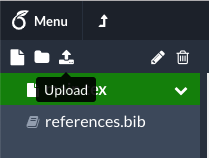
\includegraphics[scale=0.5]{overleafUpload.png}
\end{center}
    \item Include an image using only \texttt{\textbackslash includegraphics\{$\cdots$\}} as in Example \ref{example:figsimple}.
    \item Resize your image (Example \ref{example:figresize}).
    \item Include your image using the figure environment (Example \ref{example:fig}).
    \item Reference your image (Example \ref{example:fig}).
\end{enumerate}

\end{acta}
\end{center}

\section{Including Bibliography/References}\label{refSection}
There are three main bibliography management packages: bibtex, natbib (a package for use with bibtex) and biblatex. This document uses biblatex, but other packages may be better depending on your reference manager (Mendeley, EndNote, JabRef) and how you're editing / compiling your .tex documents (Overleaf, Local GUI LaTeX editor/compiler, Local command line).\\

In general, including references requires a bibliography file with all entries in a standard bibtex syntax (See: references.bib and Figure \ref{fig:strogatzbib}). It is possible to copy the bibtex syntax from google scholar (Figure \ref{fig:strogatzcite}), however reference managers such as Mendeley and EndNote can also create the LaTeX bibliography file.\\

\begin{figure}[h!]
    \centering
    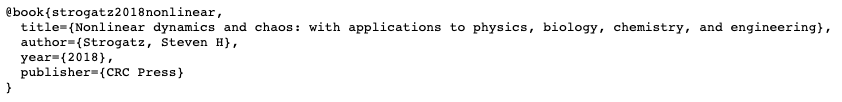
\includegraphics[width =\textwidth]{StrogatzBibTex.png}
    \caption{BibTeX entry for ``Nonlinear dynamics and chaos'' by Steven Strogatz. The bibtex key is \texttt{strogatz2018nonlinear}}
    \label{fig:strogatzbib}
\end{figure}
To cite a specific entry, type \texttt{\textbackslash cite\{$\cdots$\}} with the keyword corresponding to that entry. In Figures \ref{fig:strogatzbib} and \ref{fig:strogatzcite}, the work that should be cited (`Nonlinear dynamics and chaos'' by Steven Strogatz), has the keyword \texttt{strogatz2018nonlinear}, and is cited using the command: \texttt{\textbackslash cite\{strogatz2018nonlinear\}}. 

In Example \ref{example:michment}, the work cited (``The kinetics of the inversion effect'' by Leonor Michaelis and Maude L Menten), had the keyword \texttt{michaelis1913kinetics}, and was cited using the command: \verb!\cite{michaelis1913kinetics}!.

Print a list of the references used with the command \texttt{\textbackslash printbibliography} (Example \ref{example:michment}). 

\begin{figure}[h!]
    \centering
    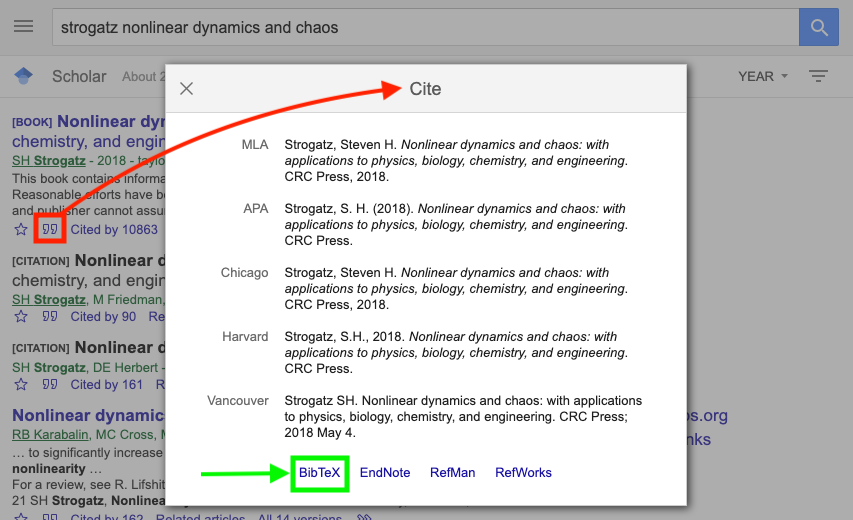
\includegraphics[width = 0.8\textwidth]{StrogatzCitationGoogle.png}
    \caption{Google Scholar Citation of `Nonlinear dynamics and chaos'' by Steven Strogatz. Clicking BibTeX will link you to Figure \ref{fig:strogatzbib}}
    \label{fig:strogatzcite}
\end{figure}

\newpage
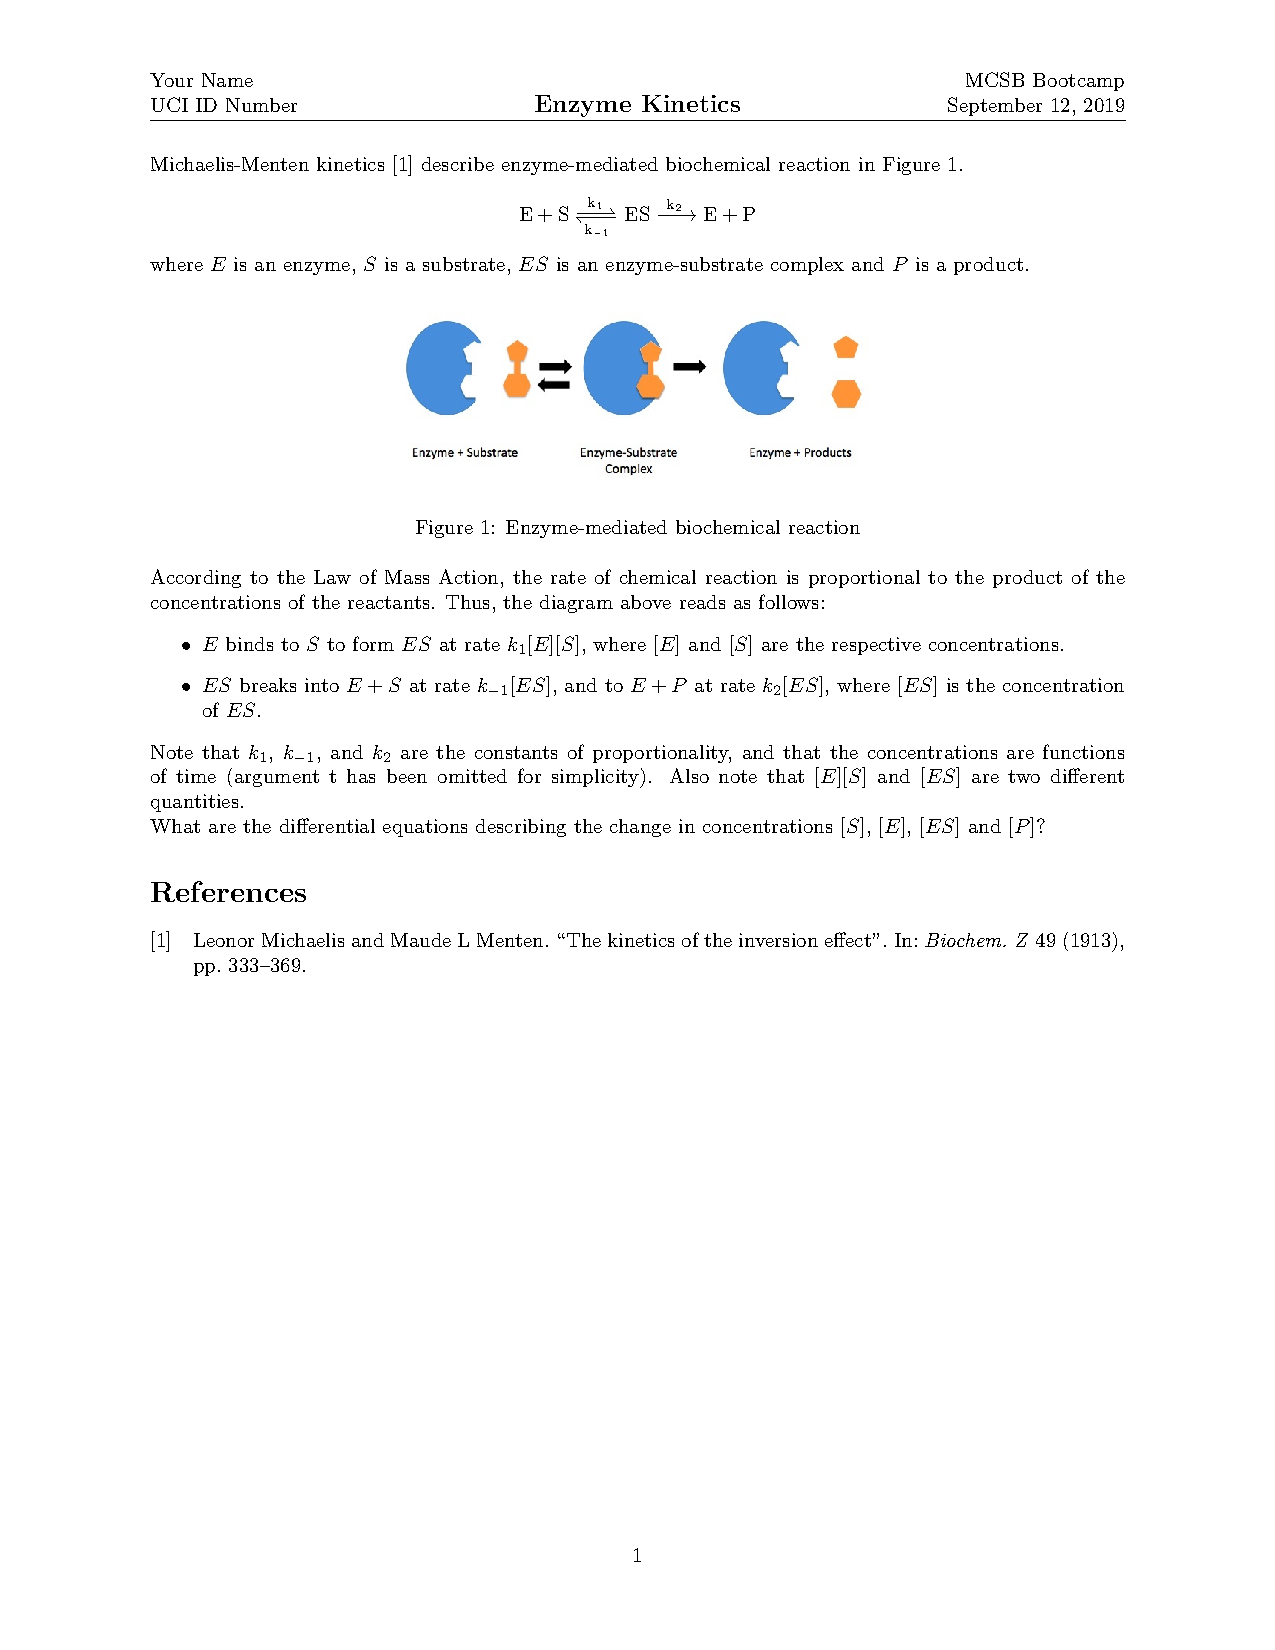
\includepdf{MCSBLatexChallenge}
\end{document}
